\section{La Carta de Smith}\label{app:carta smith}

En la Figura \ref{fig:carta smith completa} se incluye una Carta de Smith completa, pensada para imprimir y trabajar sobre ella con regla y compás. Su construcción y su uso se describen en la Sección \ref{sec:linea cargada}. Resumimos aquí el significado de sus escalas:
\begin{itemize}
    \item Las circunferencias tangentes al punto $\Gamma=1$ son las de resistencia normalizada $r$ constante, rotuladas sobre el eje real. Los arcos que parten de $\Gamma=1$ son los de reactancia normalizada $x$ constante, rotulados junto al borde: positiva (inductiva) en la mitad superior y negativa (capacitiva) en la inferior. Para ubicar una carga se normaliza $\zeta_L=Z_L/Z_0=r+jx$ y se busca la intersección correspondiente.
    \item La escala interior del borde da la fase de $\Gamma$, en grados. El módulo $|\Gamma|$ es la distancia al centro, que se mide con el compás sobre la regla inferior, donde se lee también la ROE.
    \item Las dos escalas exteriores miden desplazamientos a lo largo de la línea, en longitudes de onda. Alejarse de la carga, hacia el generador, es girar en sentido horario. Acercarse a la carga es girar en sentido antihorario. Una vuelta completa corresponde a $\lambda/2$.
    \item Para trabajar con admitancias, como en la adaptación con stub, basta con tomar el punto diametralmente opuesto y leer la misma grilla como conductancia $g$ y susceptancia $b$ normalizadas.
\end{itemize}

\begin{figure}[p]
    \begin{center}
        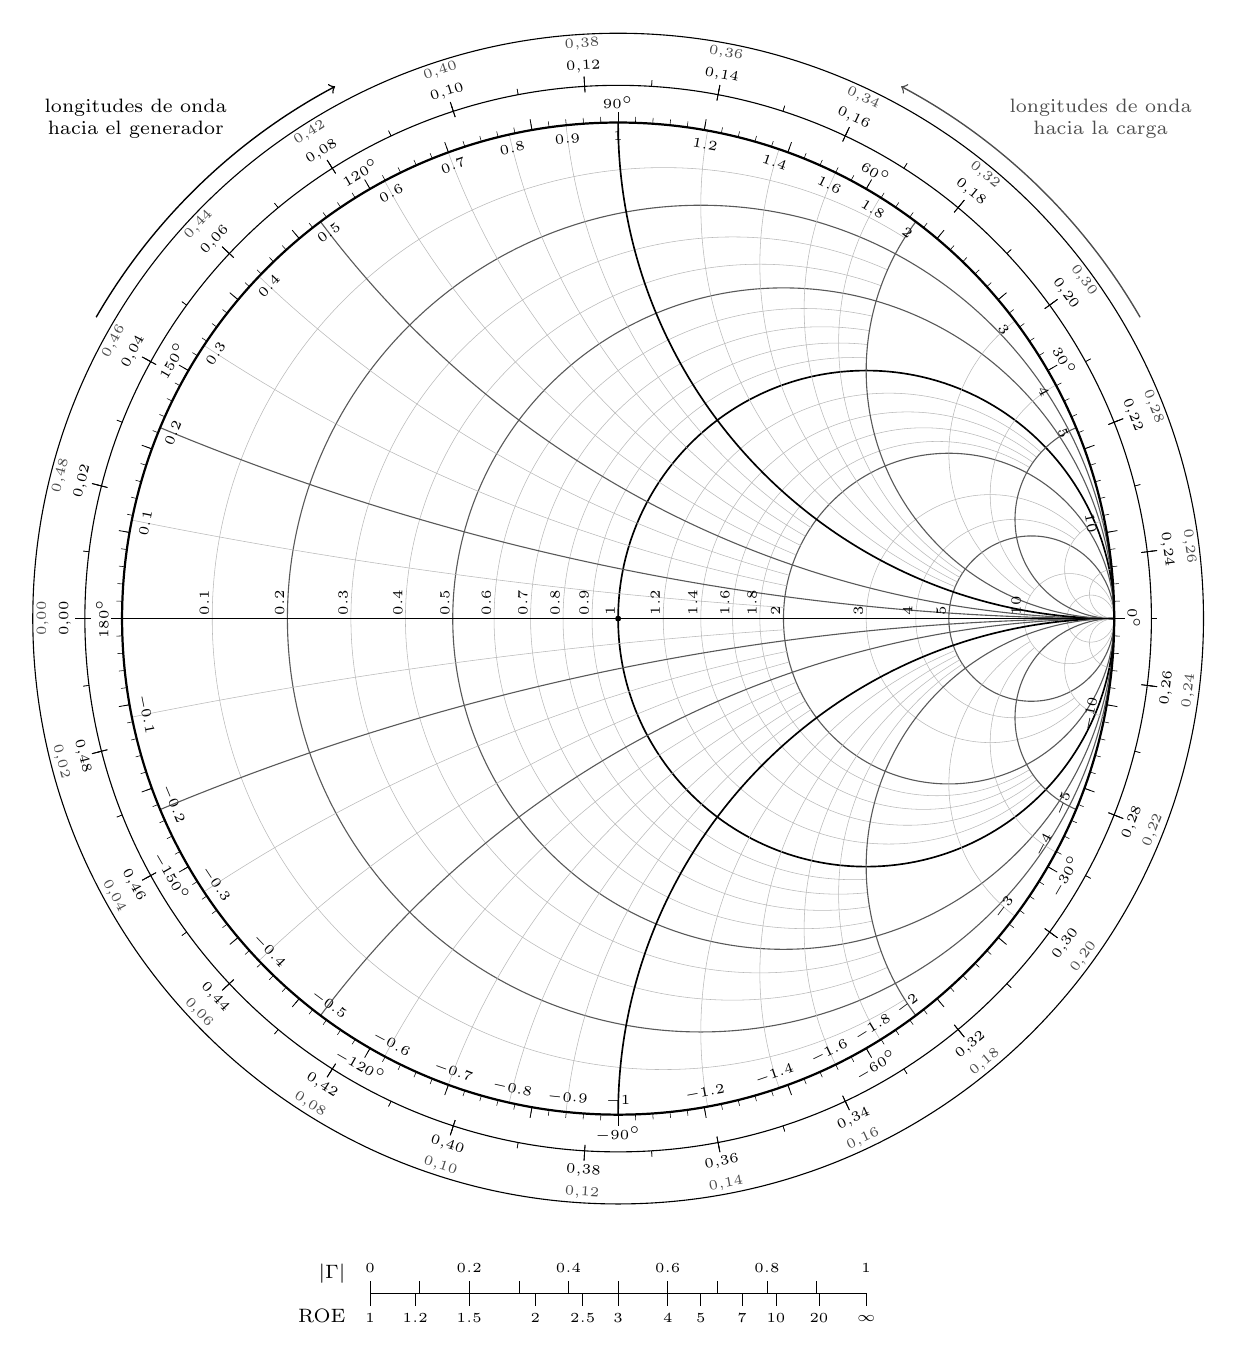
\begin{tikzpicture}[scale=6.3,
            fino/.style={gray!55, line width=0.2pt},
            medio/.style={gray!70!black, line width=0.4pt},
            grueso/.style={black, line width=0.6pt},
            ]
            % ---------------- circunferencias de r constante, truncadas en |x| <= X
            \foreach \r/\X/\estilo in {0.1/2/fino, 0.2/1000/medio, 0.3/2/fino, 0.4/2/fino, 0.5/1000/medio,
                0.6/2/fino, 0.7/2/fino, 0.8/2/fino, 0.9/2/fino, 1/1000/grueso,
                1.2/5/fino, 1.4/5/fino, 1.6/5/fino, 1.8/5/fino, 2/1000/medio,
                3/10/fino, 4/10/fino, 5/1000/medio, 10/1000/fino, 20/1000/fino}{
                \pgfmathsetmacro{\c}{\r/(\r+1)}
                \pgfmathsetmacro{\R}{1/(\r+1)}
                \pgfmathsetmacro{\ta}{180-2*atan(\X/(\r+1))}
                \pgfmathsetmacro{\tb}{180+2*atan(\X/(\r+1))}
                \draw[\estilo] ({\c+\R*cos(\ta)},{\R*sin(\ta)}) arc[start angle=\ta, end angle=\tb, radius=\R];
            }
            % ---------------- arcos de x constante, truncados en r <= Rm
            \foreach \x/\Rm/\estilo in {0.1/2/fino, 0.2/1000/medio, 0.3/2/fino, 0.4/2/fino, 0.5/1000/medio,
                0.6/2/fino, 0.7/2/fino, 0.8/2/fino, 0.9/2/fino, 1/1000/grueso,
                1.2/5/fino, 1.4/5/fino, 1.6/5/fino, 1.8/5/fino, 2/1000/medio,
                3/10/fino, 4/10/fino, 5/1000/medio, 10/1000/fino, 20/1000/fino}{
                \pgfmathsetmacro{\R}{1/\x}
                \pgfmathsetmacro{\pa}{-90-2*atan(\x/(\Rm+1))}
                \pgfmathsetmacro{\pb}{-90-2*atan(\x)}
                \draw[\estilo] ({1+\R*cos(\pa)},{\R+\R*sin(\pa)}) arc[start angle=\pa, end angle=\pb, radius=\R];
                \draw[\estilo] ({1+\R*cos(\pa)},{-\R-\R*sin(\pa)}) arc[start angle=-\pa, end angle=-\pb, radius=\R];
            }
            \draw[grueso] (-1,0) -- (1,0);
            \draw[line width=0.8pt] (0,0) circle (1);
            \fill (0,0) circle (0.006);
            % ---------------- rótulos de r, sobre el eje real
            \foreach \r in {0.1,0.2,0.3,0.4,0.5,0.6,0.7,0.8,0.9,1,1.2,1.4,1.6,1.8,2,3,4,5,10}{
                \node[rotate=90, anchor=south west, font=\tiny, inner sep=1pt] at ({(\r-1)/(\r+1)},0) {$\r$};
            }
            % ---------------- rótulos de x, junto al borde
            \foreach \x in {0.1,0.2,0.3,0.4,0.5,0.6,0.7,0.8,0.9,1,1.2,1.4,1.6,1.8,2,3,4,5,10}{
                \pgfmathsetmacro{\ang}{180-2*atan(\x)}
                \node[rotate={\ang-90}, font=\tiny, inner sep=0pt] at (\ang:0.972) {$\x$};
                \node[rotate={90-\ang}, font=\tiny, inner sep=0pt] at (-\ang:0.972) {$-\x$};
            }
            % ---------------- escala de la fase de Gamma (grados)
            \foreach \a in {0,2,...,358}{
                \draw[line width=0.2pt] (\a:1) -- (\a:1.012);
            }
            \foreach \a in {0,10,...,350}{
                \draw[line width=0.3pt] (\a:1) -- (\a:1.022);
            }
            \foreach \a in {-150,-120,-90,-60,-30,0,30,60,90,120,150,180}{
                \pgfmathsetmacro{\rot}{ifthenelse(mod(\a+720,360)<=180, \a-90, \a+90)}
                \node[font=\tiny, rotate=\rot] at (\a:1.04) {$\a^\circ$};
            }
            % ---------------- escalas en longitudes de onda
            \draw[line width=0.4pt] (0,0) circle (1.075);
            \foreach \k in {0,...,99}{
                \draw[line width=0.2pt] ({180-7.2*\k}:1.075) -- ({180-7.2*\k}:1.087);
            }
            \foreach \k in {0,...,49}{
                \draw[line width=0.3pt] ({180-14.4*\k}:1.075) -- ({180-14.4*\k}:1.095);
                \draw[line width=0.3pt] ({180-14.4*\k}:1.075) -- ({180-14.4*\k}:1.063);
            }
            \foreach \k in {0,...,24}{
                \pgfmathsetmacro{\w}{0.02*\k}
                \pgfmathsetmacro{\wl}{mod(0.5-0.02*\k,0.5)}
                \pgfmathsetmacro{\ang}{180-14.4*\k}
                \pgfmathsetmacro{\rot}{ifthenelse(mod(\ang+720,360)<=180, \ang-90, \ang+90)}
                \node[font=\tiny, rotate=\rot] at (\ang:1.115) {$\pgfmathprintnumber[fixed, fixed zerofill, precision=2, use comma]{\w}$};
                \node[font=\tiny, rotate=\rot, gray!60!black] at (\ang:1.16) {$\pgfmathprintnumber[fixed, fixed zerofill, precision=2, use comma]{\wl}$};
            }
            \draw[line width=0.4pt] (0,0) circle (1.18);
            % ---------------- sentidos de giro
            \draw[->, line width=0.5pt] (150:1.215) arc[start angle=150, end angle=118, radius=1.215];
            \node[font=\scriptsize, align=center] at (134:1.4) {longitudes de onda\\hacia el generador};
            \draw[->, line width=0.5pt, gray!60!black] (30:1.215) arc[start angle=30, end angle=62, radius=1.215];
            \node[font=\scriptsize, align=center, gray!60!black] at (46:1.4) {longitudes de onda\\hacia la carga};
            % ---------------- regla de |Gamma| y ROE
            \begin{scope}[shift={(-0.5,-1.36)}]
                \draw[line width=0.5pt] (0,0) -- (1,0);
                \foreach \g in {0,0.1,...,1.0}{
                    \draw[line width=0.3pt] (\g,0) -- (\g,0.025);
                }
                \foreach \g/\lab in {0/0, 0.2/0.2, 0.4/0.4, 0.6/0.6, 0.8/0.8, 1/1}{
                    \node[font=\tiny, above] at (\g,0.022) {$\lab$};
                }
                \foreach \s/\lab in {1/1, 1.2/1.2, 1.5/1.5, 2/2, 2.5/2.5, 3/3, 4/4, 5/5, 7/7, 10/10, 20/20}{
                    \draw[line width=0.3pt] ({(\s-1)/(\s+1)},0) -- ({(\s-1)/(\s+1)},-0.025);
                    \node[font=\tiny, below] at ({(\s-1)/(\s+1)},-0.022) {$\lab$};
                }
                \draw[line width=0.3pt] (1,0) -- (1,-0.025) node[font=\tiny, below] {$\infty$};
                \node[font=\scriptsize, anchor=east] at (-0.03,0.04) {$|\Gamma|$};
                \node[font=\scriptsize, anchor=east] at (-0.03,-0.045) {ROE};
            \end{scope}
        \end{tikzpicture}
    \end{center}
    \caption{Carta de Smith. Las escalas exteriores miden el desplazamiento a lo largo de la línea en longitudes de onda, hacia el generador (sentido horario) y hacia la carga (sentido antihorario). La escala junto al borde da la fase de $\Gamma$ en grados. En la regla inferior, de la misma escala que el radio de la carta, se lee $|\Gamma|$ y la ROE correspondiente.}\label{fig:carta smith completa}
\end{figure}
